\documentclass[a4paper,12pt]{report}

\usepackage{alltt, fancyvrb, url}
\usepackage{graphicx}
\usepackage[utf8]{inputenc}
\usepackage{float}
\usepackage{xcolor}
\usepackage{hyperref}

\usepackage[italian]{babel}

\usepackage[italian]{cleveref}

\title{OOP24 - RUNWARRIOR}
\author{
    Samuele Bianchedi, Riccardo Cornacchia\\
    Francesca Gatti, Giovanni Maria Rava}
\date{\today}
\begin{document}
\maketitle
\chapter{Analisi}
\section{Descrizione e requisiti}
Il gruppo si pone come obbiettivo quello di realizzare una reinterpretazione del famoso gioco 
Super Mario Bross del 1986. Il gioco consiste in un personaggio principale, un cavaliere, che tramite 
l'input dell'utente si muove in una mappa 2D. L'obbiettivo del cavaliere è salvare una princessa tenuta
prigioniera da uno stregone, completando diversi livelli che lo condurranno al castello nel quale è 
prigioniera. Nel gioco sarà possibile, tramite un menù, selezionare di giocare con un altro personaggio, 
un mago, che ha lo stesso obbiettivo del cavaliere. All'interno del gioco, oltre a diversi ostacoli, sono presenti nemici che il 
cavaliere deve uccidere per ottenere potenziamenti quali un armatura e la spada.
\subsection*{Requisiti funzionali}
\begin{itemize}
    \item Il personaggio deve avanzare, indietreggiare e saltare all'interno della mappa. Deve gestire le collisioni con nemici e ostacoli.
    \item Il personaggio può ottenere due potenziamenti, un'armatura e una spada che lo aiuteranno nella sua avventura.
    \item Gestione di nemici ed ostacoli diversi in base alla mappa.
    \item Creazione di un sistema di punteggio. Il punteggio verrà mostrato al completamento del livello.
\end{itemize}
\newpage
\subsection*{Requisiti non funzionali}
\begin{itemize}
    \item Implementazioni di una quarta mappa. 
    \item Gestione di restart e checkpoint.
    \item Musica e suoni. 
\end{itemize}
\section{Modello del Dominio}
RunWarrior è gioco ambientato in un mondo fantastico in cui il personaggio principale deve affrontare 3 livelli diversi. In questi
livelli il personaggio deve portersi muovere per soppravvivere e uccidere i nemici. Il movimento del personaggio è gestito tramite tastiera.
All'interno della mappa sono posizionate delle uova che racchiudono al loro interno i 2 possibili powerup (diversi per Warrior e Wizard).
Quando l'uovo viene aperto il personaggio può prendere il potenziamento successivo, quindi anche una ulteriore vita.
Per il completamento del gioco è neccessario sbloccare tutti i livelli in maniera sequenziale.
Il passaggio tra un livello e l'altro avviene tramite l'ingresso in un portale 
All'interno di ogni livello possono essere presenti degli ostacoli (MapElement) e dei nemici (Enemy) con il quale il personaggio può collidere.
Gli ostacoli possono essere: letali, non letali. I nemici sono di 5 tipi:
\begin{itemize}
    \item Goblin
    \item Snake
    \item Wizard
    \item Monkey 
    \item Guard
\end{itemize}

\begin{figure}
    \centering
    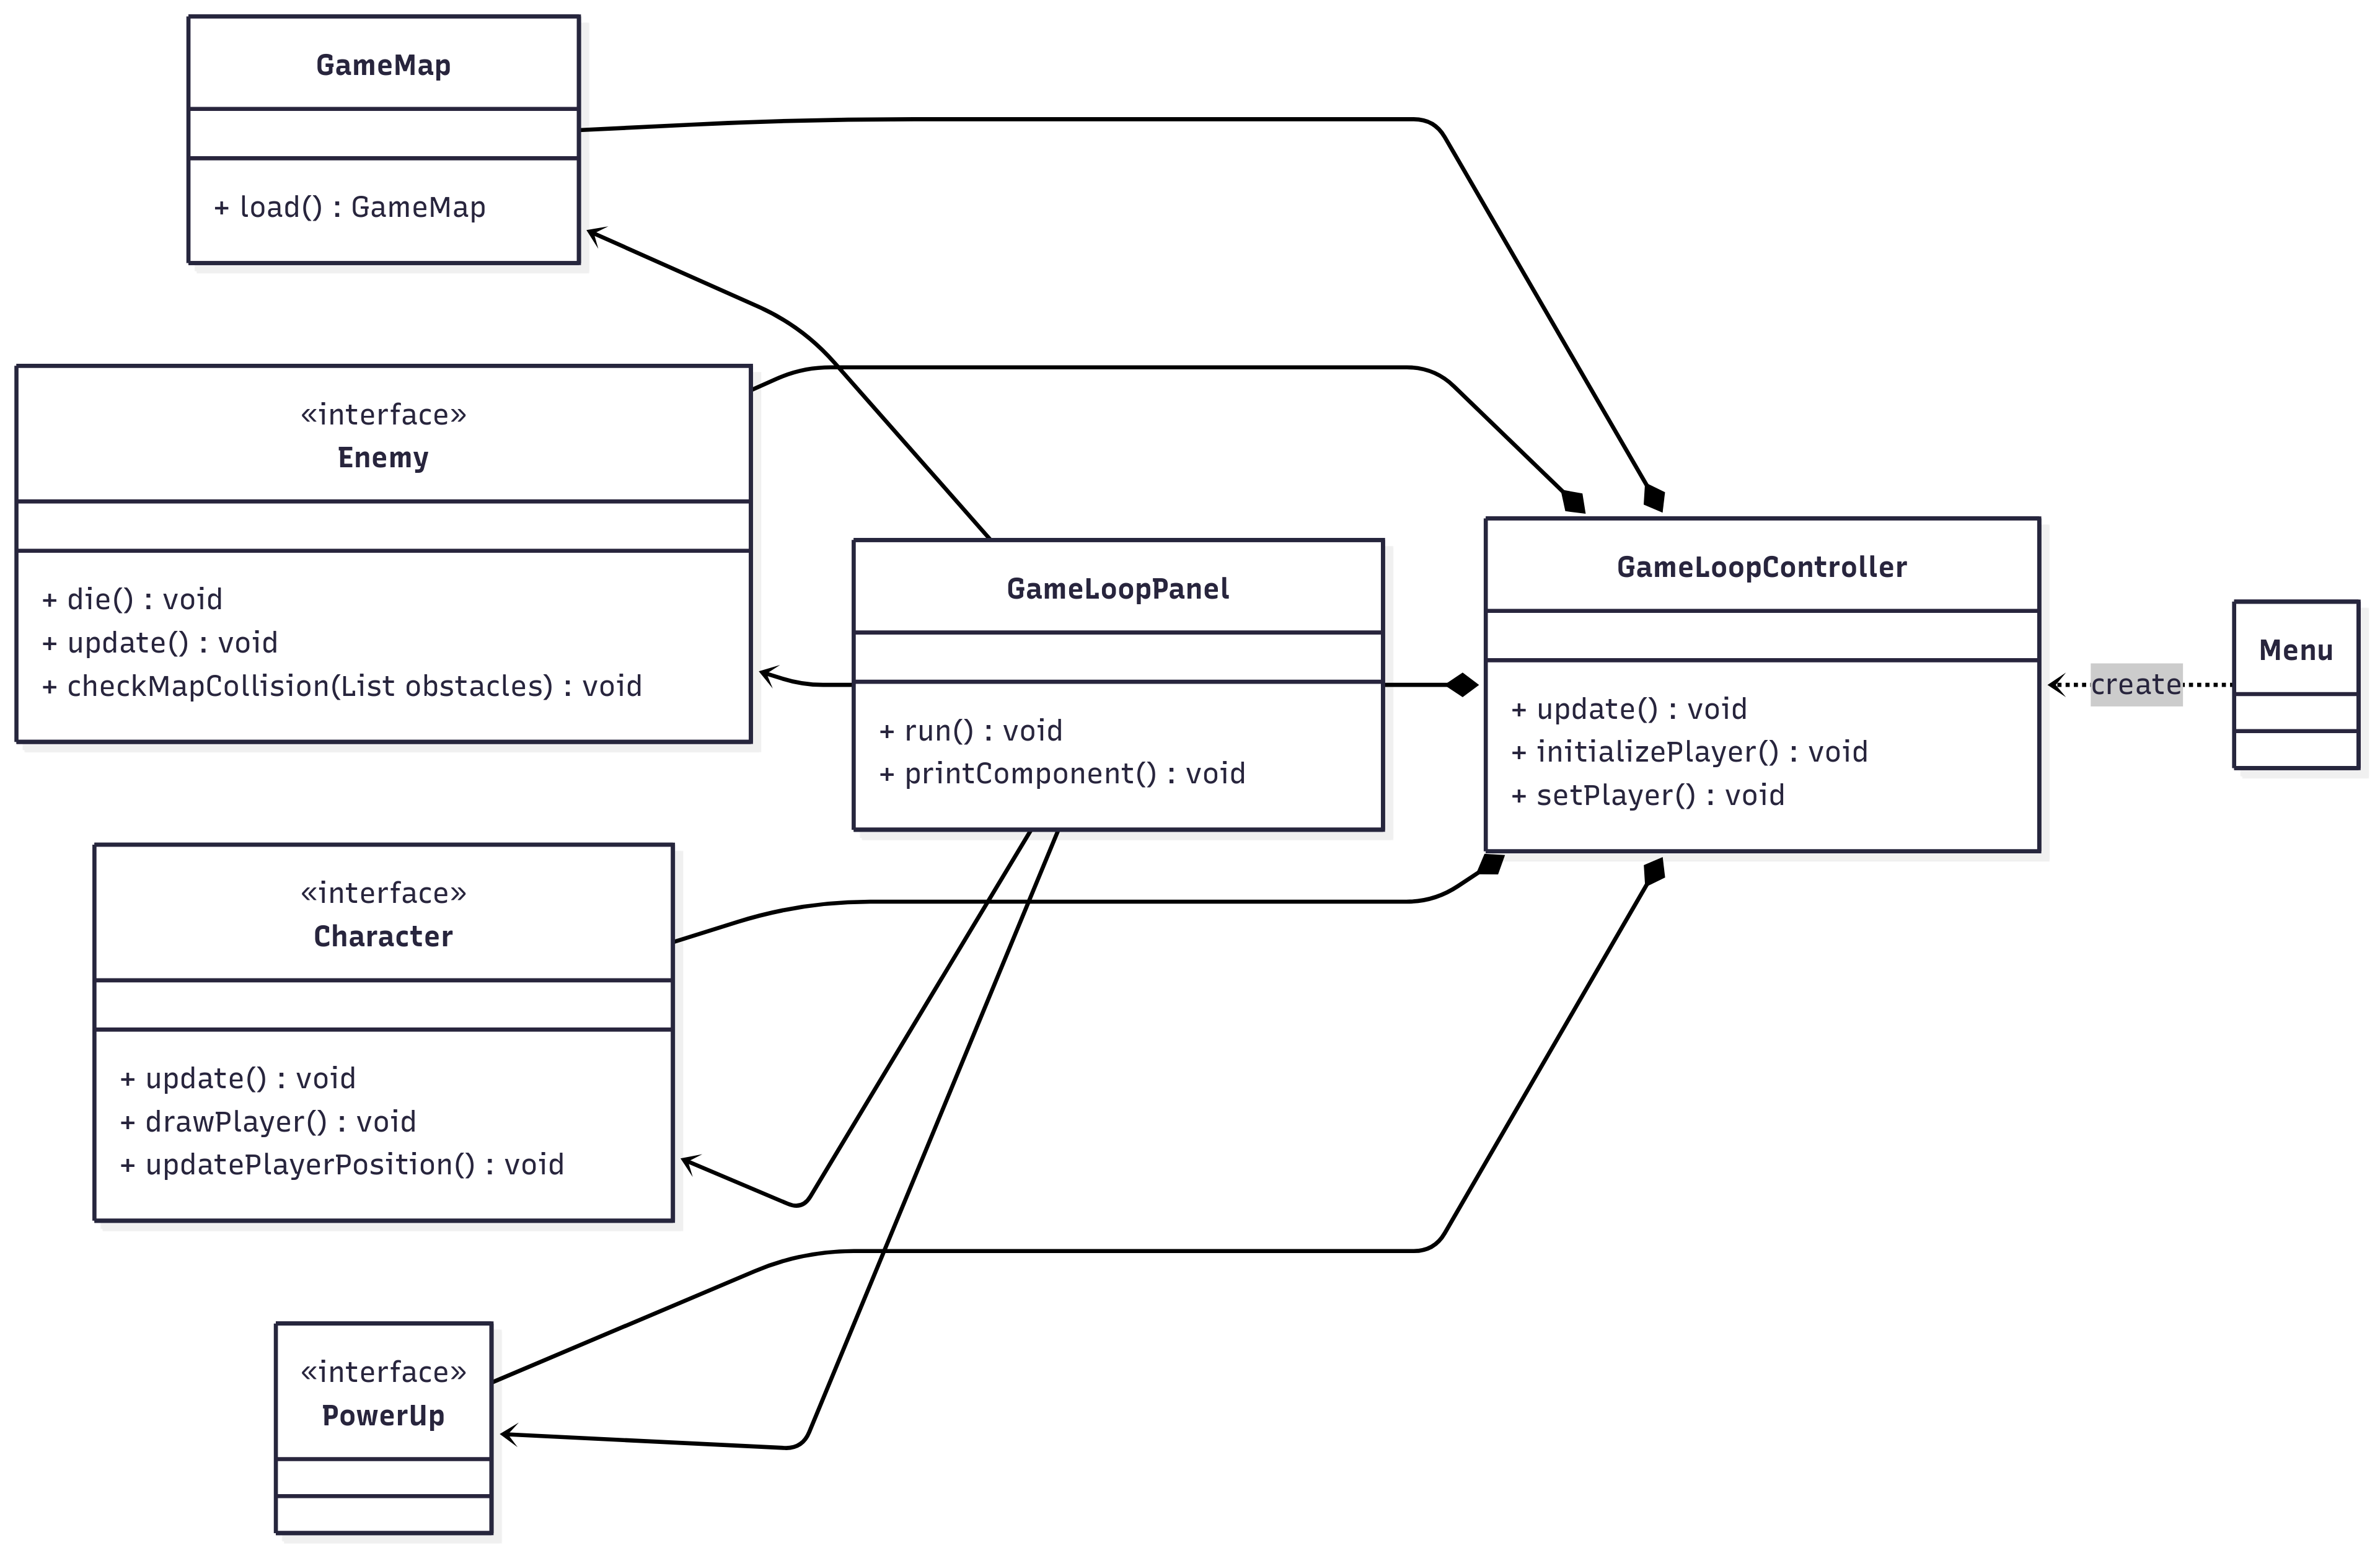
\includegraphics[width=\textwidth]{resources/modelloDominioUML.png}
    \caption{UML del modello del dominio}
    \label{}
\end{figure}

Se il personaggio collide con un ostacolo letale o con un nemico perde un potenziamento, nel caso lo avesse, altrimenti la partita finisce.
\end{document}